The metrics for our experiments are available in table 1. The scores are very high for Accuracy, Recall, F1Score and Precision (>= 90), we even 
have for ConvLSTM 53\% exact matches, which means that the predicted image was exactly the ground truth that occurred.
however this does not mean that the model is correct, due to a very high data imbalance towards 0 or no rain in the dataset.
The most important metric that actually quantifies the performance of the model is the Jaccard Index. The best performing model following this metric is the plain ConvLSTM model
with a Convolutional head. If we compare both U-Net and ConvLSTM models visually \ref{fig:convclass} \ref{unet} we can see that ConvLSTM is more confident in predicting high rain intensity
while the U-Net model predicts only low levels of rain, however it is more accurate at predicting the area of rain in the ground truth. Another remark is that all metrics seem to be the same across the models.
This can occur if the false positive rate is equal to the false negative rate.

\begin{table*}[]
  \caption[short]{Metrics on Test Set for variants of classification models trained on 50 epochs.}
  \begin{tabular}{@{}lllllll@{}}
  \toprule
  Models               & Accuracy & Precision & Recall & F1Score & Exact Match & Jaccard Index \\ \midrule
  3D U-Net                & 0.9199   & 0.9199    & 0.9199 & 0.9199  & 0.0000      & 0.1150        \\
  ConvLSTM             & 0.9999   & 0.9999    & 0.9999 & 0.9999  & 0.5385      & 0.1249        \\
  ConvLSTM + Attention & 0.9300   & 0.9300    & 0.9300 & 0.9300  & 0.0000      & 0.1160 
  \end{tabular}
\end{table*}


\begin{figure*}[hbp]
  \centering
  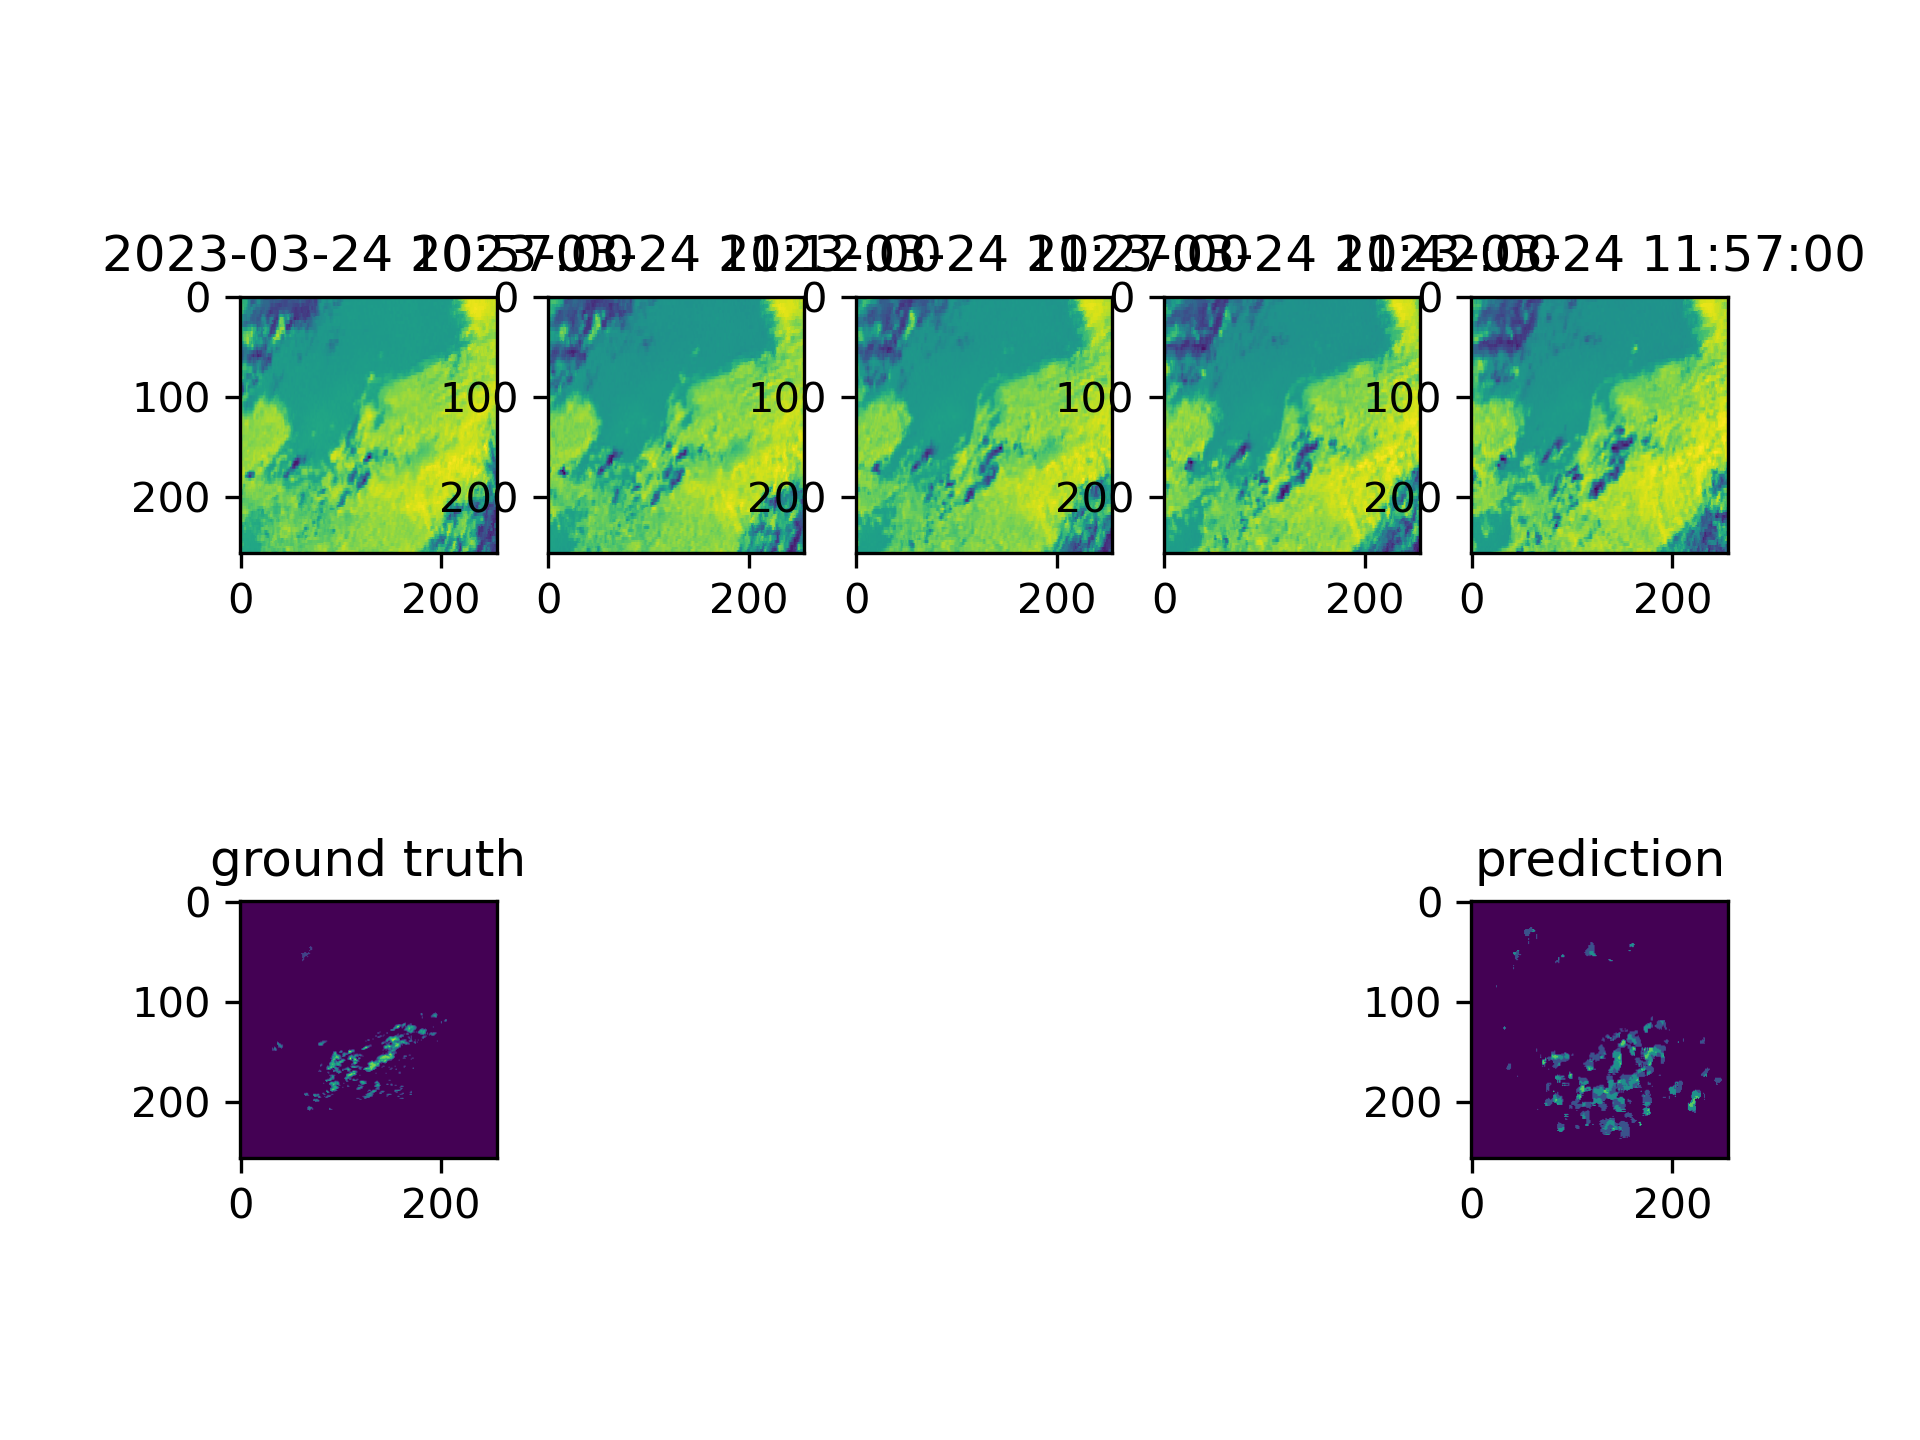
\includegraphics[width=225pt]{./images/experiment-0.png}
  \caption{Testset prediction with ConvLSTM model for 2023-03-24 12:02:00 UTC.}
  \Description{}
  \label{fig:convclass}
\end{figure*}

\begin{figure*}[hbp]
  \centering
  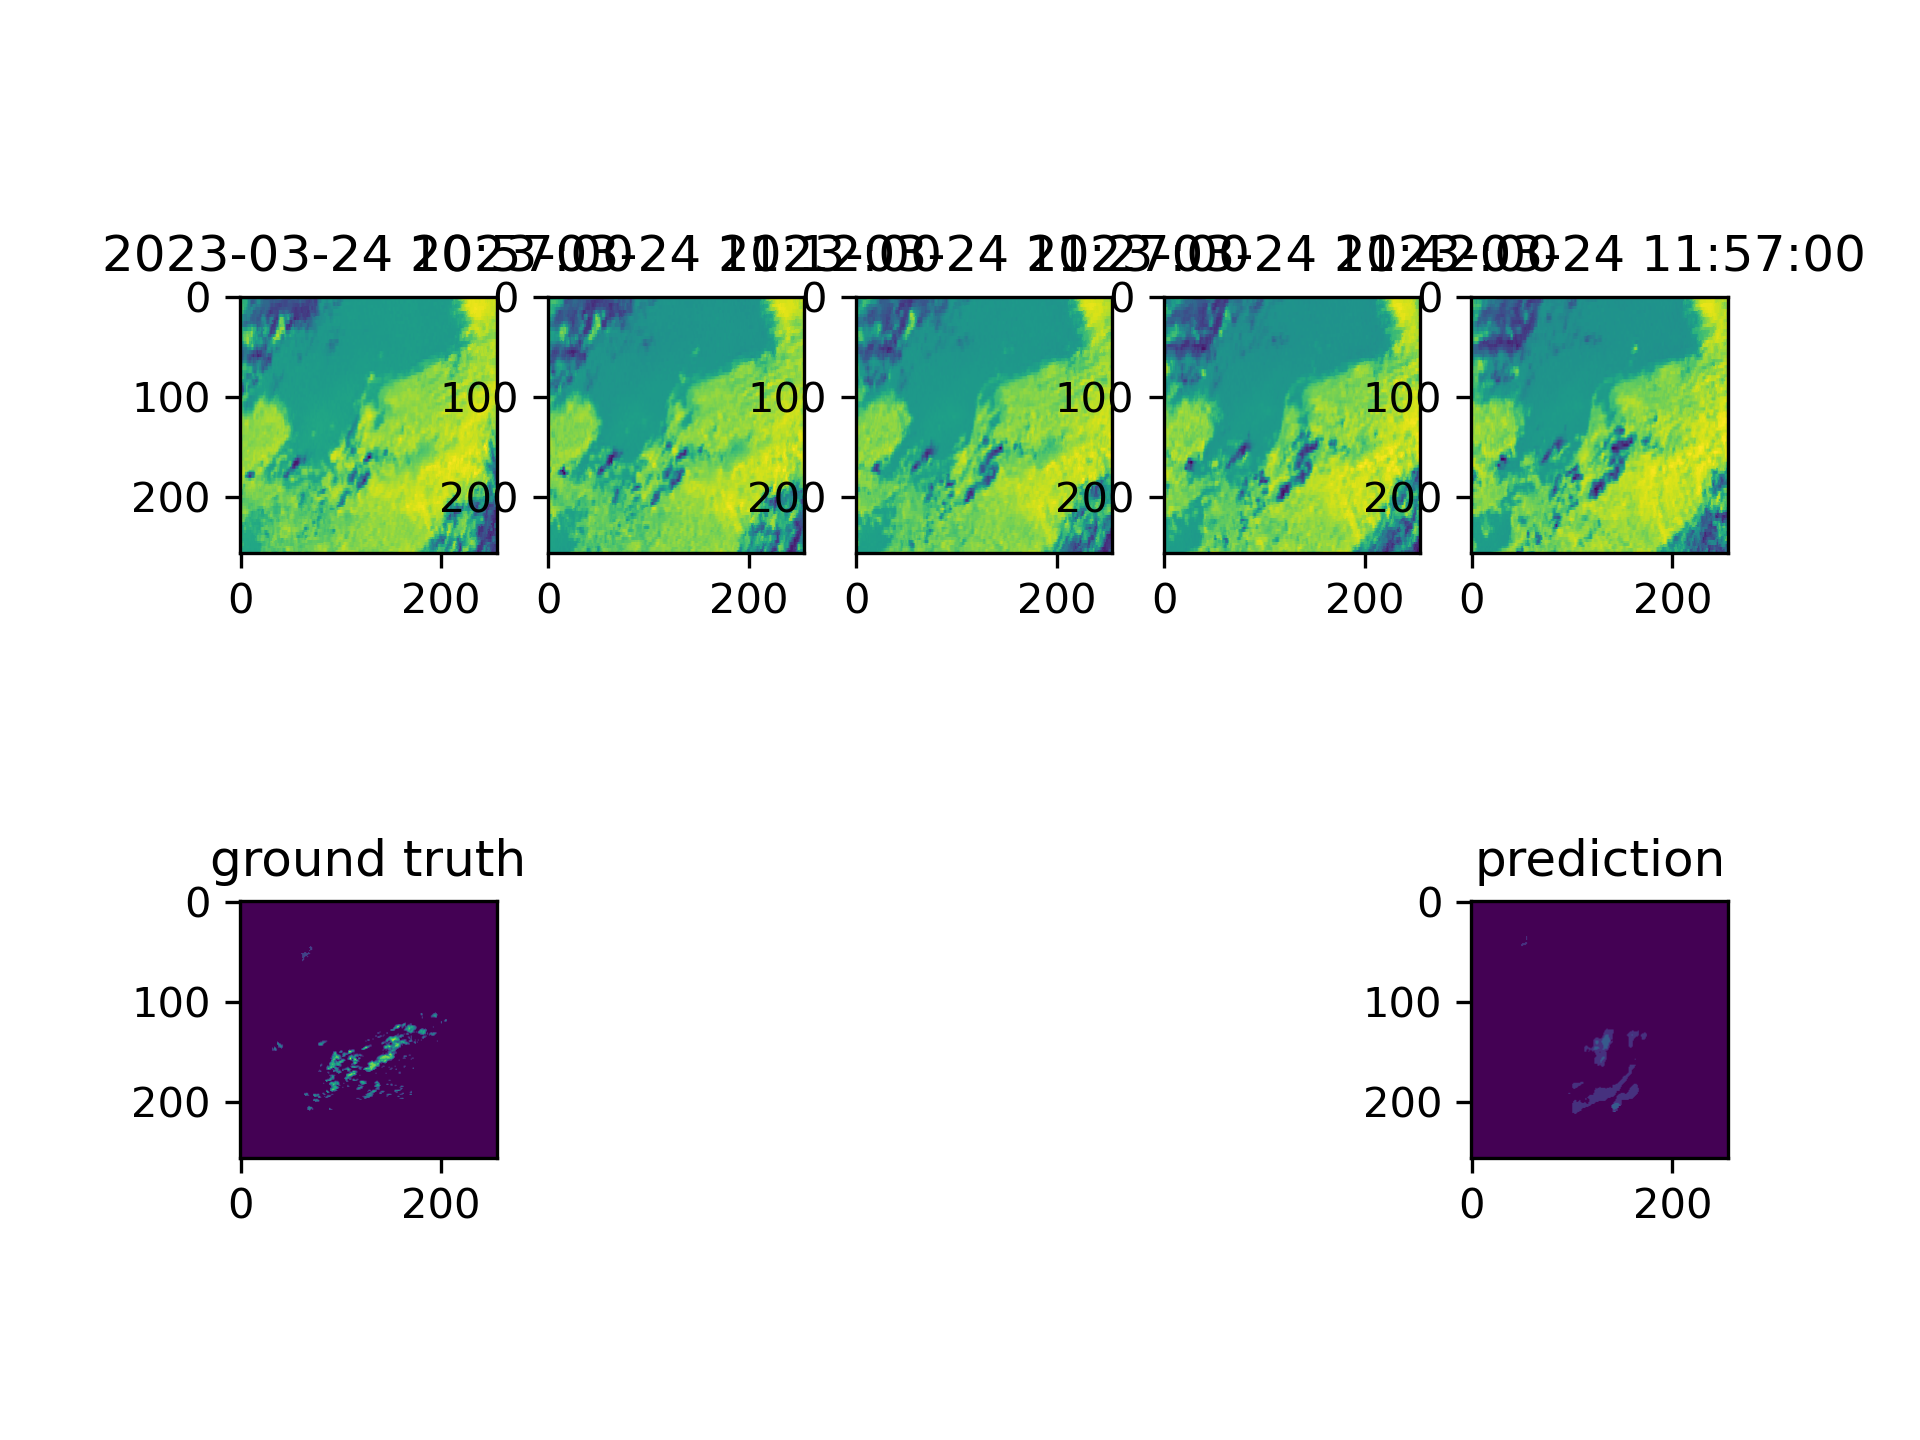
\includegraphics[width=225pt]{./images/experiment-0-unet.png}
  \caption{Testset prediction with U-Net model for 2023-03-24 12:02:00 UTC.}
  \Description{}
  \label{fig:unet}
\end{figure*}